% Just The Docs Front Matter
% title: Modeling Helheim Glacier
% parent: Tutorials
% has_children: false
% has_toc: false

\subsection{Modeling Helheim Glacier} \label{sec:using-issm-tutorials-helheim}
\subsubsection{Goals}
\begin{itemize}
	\item Create an ice-flow model of Helheim Glacier (southeast Greenland)
	\item Run an inversion model to infer basal friction
\end{itemize}

\subsubsection{Introduction}
In this example, the main goal is to parameterize and model a real Greenland outlet glacier. In order to build an operational simulation of Helheim Glacier, we will follow these steps:
\begin{itemize}
	\item Define the model region
	\item Create a mesh
	\item Parameterize the model
	\item Invert for friction coefficient
	\item Plot results
\end{itemize}

Files needed for this tutorial can be found in \lstinlinebg|<ISSM_DIR>/examples/Helheim/|. The \lstinlinebg|runme.m| file contains the structure of the simulation, while the \lstinlinebg|.par| file includes most parameters needed for the model set-up. The \lstinlinebg|.exp| file contains coordinates that define the model domain boundaries.

Observed datasets needed for the parameterization need to be downloaded.

\subsubsection{Mesh}
The first step is to create the model domain outline and mesh.

In the \lstinlinebg|runme.m| file, the mesh is generated in a multi-step process. Open the \lstinlinebg|runme.m| file and make sure that the variable \lstinlinebg|steps|, at the top of the file, is set to \lstinlinebg|steps = [1]|. In the code, you will see that in Step 1 the following actions are implemented:

\begin{itemize}
	\item Create a uniform mesh
	\item Refine the mesh using anisotropic mesh refinement based on surface velocity
	\item Set the mesh parameters
	\item Load observed surface velocities
	\item Interpolate velocity onto a coarse mesh. Adapt the mesh to minimize error in velocity interpolation
	\item Save the model
\end{itemize}

Execute the \lstinlinebg|runme.m| file to perform step 1. Plot the mesh with:

\begin{lstlisting}
plotmodel(md, 'data', 'mesh')
\end{lstlisting}

You should see the following figure, with finer resolution in the two main branches of Helheim and its main trunk:
\begin{figure}[h!]
	\begin{center}
	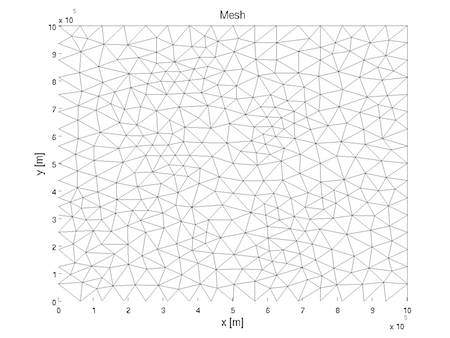
\includegraphics[width=\textwidth]{\assetsParentPath/assets/img/using-issm/tutorials/helheim/mesh.png}
	\end{center}
\end{figure}

Try experimenting with different values in the mesh generation to create finer or coarser meshes.

\subsubsection{Parameterization}
Most of the model parameterization is done through a different file (\lstinlinebg|Greenland.par|). In this example, we parameterize the following model fields:
\begin{itemize}
	\item Geometry (ice surface elevation and bed topography, using BedMachine)
	\item Initialization parameters
	\item Material parameters
	\item Friction coefficient
	\item Boundary conditions
\end{itemize}

Run step 2 in the \lstinlinebg|runme.m| file to perform the parameterization.

\subsubsection{Inversion for basal friction}%{{{
The friction coefficient is inferred from the surface velocity using the following friction law:
\begin{equation}
	\mathbf{ \tau }_b = -\beta^{2} N^r \|\mathbf{v_b}\|^{s-1}\mathbf{v_b}
\end{equation}

\begin{itemize}
	\item $\mathbf{ \tau }_b$ : Basal stress (basal drag)
	\item $N$: Effective pressure (ice overburden pressure - water pressure at the bed)
	\item $v_b$: Basal velocity (equal to surface velocity in SSA approximation)
	\item $r$: Exponent (equals $q/p$ of the parameter file)
	\item $s$: Exponent (equals $1/p$ of the parameter file)
\end{itemize}

The procedure for the inversion is as follows:
\begin{itemize}
	\item Velocity is computed from the SSA approximation
	\item Misfit of the cost function is computed
	\item Friction coefficient is modified following the gradient of the cost function
\end{itemize}

All the parameters that can be adjusted for the inversion are in \lstinlinebg|md.inversion|.

Run step 3. This will take a few minutes to run. Plot the resulting velocity and friction coefficient:

\begin{lstlisting}
plotmodel(md, 'data', md.initialization.vel, 'title', 'Surface Velocity (m/yr)', ...
	'data', md.friction.coefficient, 'title', 'Friction Coefficient')
\end{lstlisting}
You should see something similar to the figure below:
\begin{figure}[h!]
	\begin{center}
		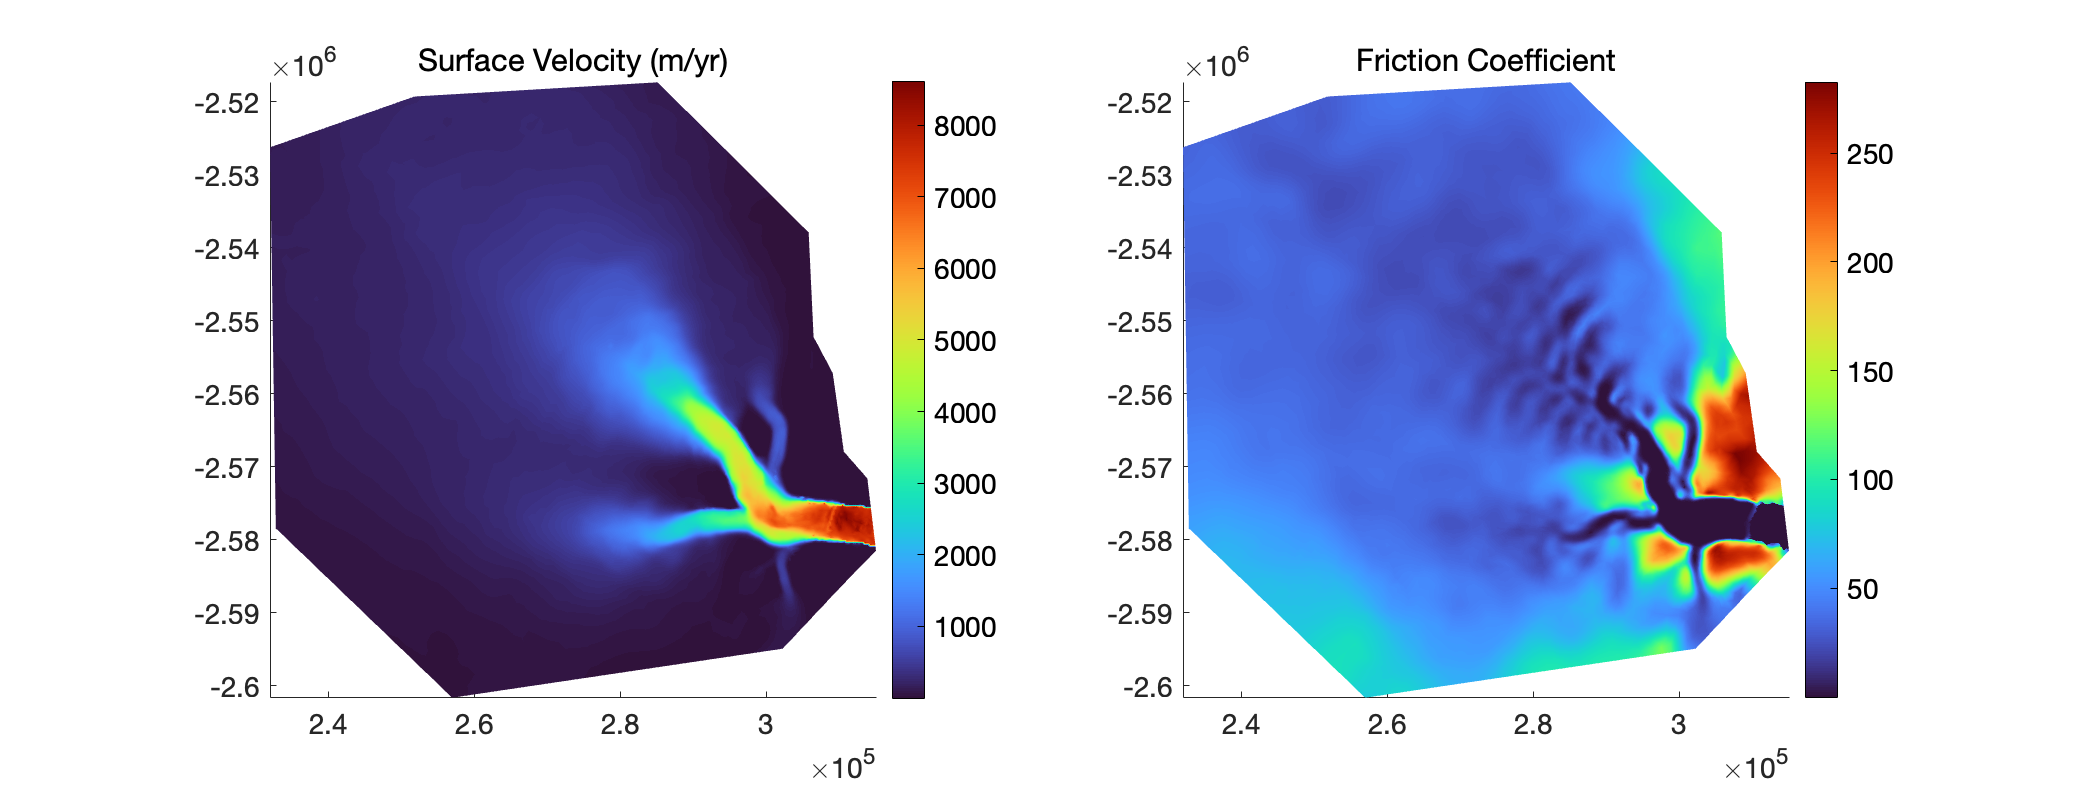
\includegraphics[width=\textwidth]{\assetsParentPath/assets/img/using-issm/tutorials/helheim/figure_vel_fric.png}
	\end{center}
\end{figure}

Try experimenting with different cost-function values and other parameters in \lstinlinebg|md.inversion|.

Now that you have run an inversion for basal friction and have a working stress-balance model of Helheim Glacier, you are ready for the next tutorial on simulating subglacial hydrology at Helheim using the SHAKTI model.

\clearpage % Make sure all figures are placed before next section
